\documentclass[12pt,addpoints]{repaso}
\grado{5}
\nivel{Primaria}
\cicloescolar{2024-2025}
\materia{Matemáticas}
\unidad{
	2}
\title{Practica la Unidad}
\aprendizajes{\scriptsize%
	% \item Estudio de los números.
\item Ordena, lee, escribe e identifica regularidades en números naturales de hasta nueve cifras. Lee, escribe y ordena números decimales hasta diezmilésimos en notación decimal y letra, y los interpreta en diferentes contextos.
	% \item Suma y resta, su relación como operaciones inversas.
	\item Propone y resuelve situaciones problemáticas que implican sumas y restas con números decimales utilizando el algoritmo convencional y fracciones con diferentes denominadores. 
	% \item Multiplicación y división, su relación como operaciones inversas.
	\item Resuelve situaciones problemáticas vinculadas a diferentes contextos que implican multiplicar números fraccionarios y números decimales, con un número natural como multiplicador.También, dividir números naturales y el cociente resulte un número decimal.
	% \item Relaciones de proporcionalidad.
	\item Resuelve situaciones problemáticas de proporcionalidad en las que determina valores faltantes de números naturales, a partir de diferentes estrategias (cálculo del valor unitario, de dobles, triples o mitades).
	% \item Ubicación espacial.
	\item Elabora e interpreta croquis para comunicar la ubicación de seres vivos, objetos, trayectos o lugares.
	% \item Medición de la longitud, masa y capacidad.
	% \item Figuras y cuerpos geométricos y sus características.
	\item Reconoce y describe semejanzas y diferencias entre un prisma y una pirámide; propone desarrollos planos para construir prismas rectos cuadrangulares o rectangulares.
	% \item Perímetro, área y noción de volumen.
	\item Calcula el perímetro y área de diferentes polígonos. Construye y usa fórmulas para calcular el perímetro de cualquier polígono, a partir de sumar la longitud de todos sus lados o multiplicar el número de lados por la medida de uno de ellos.
	% \item Organización e interpretación de datos.
	\item Construye tablas y gráficas de barras, e interpreta información cuantitativa y cualitativa contenida en ellas.
	% \item Nociones de probabilidad. 
	\item Identifica situaciones de distintos contextos en las que interviene o no el azar; registra resultados de experiencias aleatorias en tablas de frecuencias y expresa la frecuencia absoluta y la relativa.
	  }
\author{Melchor Pinto, JC}
\begin{document}
\INFO
\begin{multicols}{2}
	\tableofcontents
\end{multicols}
\begin{questions}\large
	\addcontentsline{toc}{section}{Unidad 2}
	\section*{Unidad 2}

	\addcontentsline{toc}{subsection}{Números decimales}
	\subsection*{Números decimales}
	% \subsection*{\ifprintanswers{Posición decimal y notación desarrollada}

	\questionboxed[2]{Escribe los siguientes números

		\begin{multicols}{2}
			\begin{parts}\normalsize
				\part Catorce enteros diecinueve centésimos 	\hfill \fillin[14.19][1.2cm]
				\part Cuatro enteros once diez milésimos 		\hfill \fillin[4.0011][1.2cm]
				\part Seis enteros setenta y dos centésimos 	\hfill \fillin[6.72][1.2cm]
				\part Siete enteros novecientos tres milésimos 	\hfill \fillin[7.903][1.2cm]
				\part Seis enteros doscientos trece milésimos 	\hfill \fillin[6.213][1.2cm]
				\part Cincuenta enteros cinco décimos 			\hfill \fillin[50.5][1.2cm]
				\part Nueve enteros cuatro centésimos 			\hfill \fillin[9.04][1.2cm]
				\part Cuatro enteros setecientos doce milésimos \hfill \fillin[4.712][1.2cm]
				\part Seis mil catorce diez milésimos 			\hfill \fillin[0.6014][1.2cm]
				\part Nueve enteros once centésimos 			\hfill \fillin[9.11][1.2cm]
				\part Cuarenta enteros cuatro centésimos 		\hfill \fillin[40.04][1.2cm]
				\part Dieciocho enteros siete décimos 			\hfill \fillin[18.7][1.2cm]
				\part Veinte enteros tres décimos 				\hfill \fillin[20.3][1.2cm]
				\part Cuatro enteros ciento dos diez milésimos 	\hfill \fillin[4.0102][1.2cm]
				\part Ocho enteros trece diez milésimos 		\hfill \fillin[8.0013][1.2cm]
			\end{parts}
		\end{multicols}
	}

	\questionboxed[2]{Señala la opción que responda correctamente a cada una de las siguientes preguntas:

		\begin{multicols}{2}
			\begin{parts}
				\part En el número 1.829, ¿qué número ocupa la posición de las centésimas?

				\begin{oneparcheckboxes}
					\choice 1 \CorrectChoice 2 \choice 6 \choice 8 \choice 9
				\end{oneparcheckboxes}

				\part En el número 2.087, ¿qué número ocupa la posición de las décimas?

				\begin{oneparcheckboxes}
					\CorrectChoice 0 \choice 2 \choice 7 \choice 8 \choice 9
				\end{oneparcheckboxes}

				\part En el número 5.928, ¿qué número ocupa la posición de las décimas?

				\begin{oneparcheckboxes}
					\choice 5 \choice 2 \choice 6 \choice 8 \CorrectChoice 9
				\end{oneparcheckboxes}

				\part En el número 3.284, ¿qué número ocupa la posición de las milésimas?

				\begin{oneparcheckboxes}
					\choice 2 \choice 3 \CorrectChoice 4  \choice 8 \choice 9
				\end{oneparcheckboxes}

				\part En el número 1.285, ¿qué número ocupa la posición de las décimas?

				\begin{oneparcheckboxes}
					\choice 1 \CorrectChoice 2 \choice 5 \choice 8 \choice 9
				\end{oneparcheckboxes}

				\part En el número 1.823, ¿qué número ocupa la posición de las milésimas?

				\begin{oneparcheckboxes}
					\choice 1 \choice 2 \CorrectChoice 3 \choice 6 \choice 8
				\end{oneparcheckboxes}
			\end{parts}
		\end{multicols}
	}


	% \subsection*{\ifprintanswers{Suma de decimales            }\else{}\fi}
	\questionboxed[2]{Realiza las siguientes sumas con números decimales:

		\begin{multicols}{3}
			\begin{parts}
				\part \ifprintanswers{   \opadd[hfactor=decimal,resultstyle=\color{red},carryadd=true,carrysub=false]{24.34}{13.84} }
				\else{            \opadd[hfactor=decimal,resultstyle=\color{white},carryadd=false,carrysub=false]{24.34}{13.84}\\[0.5cm]}
				\fi

				\part \ifprintanswers{   \opadd[hfactor=decimal,resultstyle=\color{red},carryadd=true,carrysub=false]{684.99}{583.82} }
				\else{           \opadd[hfactor=decimal,resultstyle=\color{white},carryadd=false,carrysub=false]{684.99}{583.82} \\[0.5cm]}
				\fi

				\part \ifprintanswers{   \opadd[hfactor=decimal,resultstyle=\color{red},carryadd=true,carrysub=false]{51.238}{34.993} }
				\else{            \opadd[hfactor=decimal,resultstyle=\color{white},carryadd=false,carrysub=false]{51.238}{34.993}\\[0.5cm] }
				\fi

				\part \ifprintanswers{   \opadd[hfactor=decimal,resultstyle=\color{red},carryadd=true,carrysub=false]{90.371}{45.392} }
				\else{            \opadd[hfactor=decimal,resultstyle=\color{white},carryadd=false,carrysub=false]{90.371}{45.392} \\[0.5cm]}
				\fi

				\part \ifprintanswers{   \opadd[hfactor=decimal,resultstyle=\color{red},carryadd=true,carrysub=false]{18.03}{7.45} }
				\else{            \opadd[hfactor=decimal,resultstyle=\color{white},carryadd=false,carrysub=false]{18.03}{7.45}\\[0.5cm] }
				\fi

				\part \ifprintanswers{   \opadd[hfactor=decimal,resultstyle=\color{red},carryadd=true,carrysub=false]{9.931}{5.198} }
				\else{           \opadd[hfactor=decimal,resultstyle=\color{white},carryadd=false,carrysub=false]{9.931}{5.198}\\[0.5cm] }
				\fi
			\end{parts}
		\end{multicols}
	}

	% \subsection*{\ifprintanswers{Resta de decimales           }\else{}\fi}

	\questionboxed[2]{Realiza las siguientes restas con números decimales:

		\begin{multicols}{3}
			\begin{parts}
				\part \ifprintanswers{   \opsub[hfactor=decimal,resultstyle=\color{red},carryadd=true,carrysub=true]{9.754}{3.862} }
				\else{            \opsub[hfactor=decimal,resultstyle=\color{white},carryadd=false,carrysub=false]{9.754}{3.862}\\[0.5cm]}
				\fi

				\part \ifprintanswers{   \opsub[hfactor=decimal,resultstyle=\color{red},carryadd=true,carrysub=true]{1.668}{1.464} }
				\else{            \opsub[hfactor=decimal,resultstyle=\color{white},carryadd=false,carrysub=false]{1.668}{1.464} \\[0.5cm]}
				\fi

				\part \ifprintanswers{   \opsub[hfactor=decimal,resultstyle=\color{red},carryadd=true,carrysub=true]{4.298}{3.465} }
				\else{            \opsub[hfactor=decimal,resultstyle=\color{white},carryadd=false,carrysub=false]{4.298}{3.465}\\[0.5cm] }
				\fi

				\part \ifprintanswers{   \opsub[hfactor=decimal,resultstyle=\color{red},carryadd=true,carrysub=true]{90.371}{45.392} }
				\else{            \opsub[hfactor=decimal,resultstyle=\color{white},carryadd=false,carrysub=false]{90.371}{45.392} \\[0.5cm]}
				\fi

				\part \ifprintanswers{   \opsub[hfactor=decimal,resultstyle=\color{red},carryadd=true,carrysub=true]{16.03}{6.45} }
				\else{            \opsub[hfactor=decimal,resultstyle=\color{white},carryadd=false,carrysub=false]{16.03}{6.45}\\[0.5cm] }
				\fi

				\part \ifprintanswers{   \opsub[hfactor=decimal,resultstyle=\color{red},carryadd=true,carrysub=true]{6.231}{2.188} }
				\else{            \opsub[hfactor=decimal,resultstyle=\color{white},carryadd=false,carrysub=false]{6.231}{2.188}\\[0.5cm] }
				\fi
			\end{parts}
		\end{multicols}
	}

	\questionboxed[2]{Realiza las siguientes multiplicaciones con números decimales:

		\begin{multicols}{3}
			\begin{parts}
				\part \ifprintanswers{\normalsize\opmul[hfactor=decimal,resultstyle=\color{red},displayintermediary=None]{3.24}{2.52} }
				\else{\opmul[hfactor=decimal,resultstyle=\color{white},displayintermediary=None]{3.24}{2.52}}\\[2em]\fi

				\part \ifprintanswers{\normalsize\opmul[hfactor=decimal,resultstyle=\color{red},displayintermediary=all]{7.75}{3.8} }
				\else{\opmul[hfactor=decimal,resultstyle=\color{white},displayintermediary=None]{7.75}{3.8}}\\[2em]\fi

				\part \ifprintanswers{\normalsize\opmul[hfactor=decimal,resultstyle=\color{red},displayintermediary=None]{1.9}{1.2} }
				\else{\opmul[hfactor=decimal,resultstyle=\color{white},displayintermediary=None]{1.9}{1.2}}\\[2em]\fi

				\part \ifprintanswers{\normalsize\opmul[hfactor=decimal,resultstyle=\color{red},displayintermediary=all]{2.5}{2.3} }
				\else{\opmul[hfactor=decimal,resultstyle=\color{white},displayintermediary=None]{2.5}{2.3}}\\[2em]\fi

				\part \ifprintanswers{\normalsize\opmul[hfactor=decimal,resultstyle=\color{red},displayintermediary=all]{23.4}{8.5} }
				\else{\opmul[hfactor=decimal,resultstyle=\color{white},displayintermediary=None]{23.4}{8.5}}\\[2em]\fi

				\part \ifprintanswers{\normalsize\opmul[hfactor=decimal,resultstyle=\color{red},displayintermediary=all]{5.3}{1.6} }
				\else{\opmul[hfactor=decimal,resultstyle=\color{white},displayintermediary=None]{5.3}{1.6}}\\[2em]\fi
			\end{parts}
		\end{multicols}
	}

	\addcontentsline{toc}{subsection}{Decimales y porcentajes}
	\subsection*{Decimales y porcentajes}
	% \subsection*{\ifprintanswers{Decimales en la recta númerica        }
	\questionboxed[2]{Escribe en el recuadro el número decimal que representa el punto en la recta numérica de cada imagen:

		\begin{multicols}{2}
			\begin{parts}
				\part 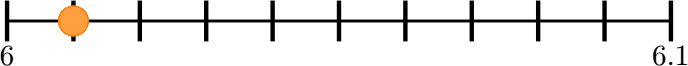
\includegraphics[width=180px]{../images/recta_num_6.01.png}  \hfill \fillin[\fbox{6.01}][0in] \\
				\part 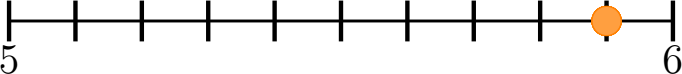
\includegraphics[width=180px]{../images/recta_num_5.9.png}   \hfill \fillin[\fbox{5.9 }][0in] \\
				\part 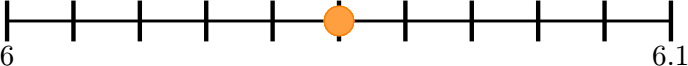
\includegraphics[width=180px]{../images/recta_num_6.05.png}  \hfill \fillin[\fbox{6.05}][0in] \\
				\part 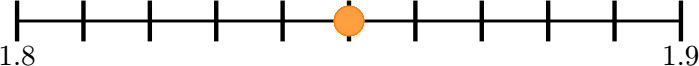
\includegraphics[width=180px]{../images/recta_num_1.85.png}  \hfill \fillin[\fbox{1.85}][0in] \\
				\part 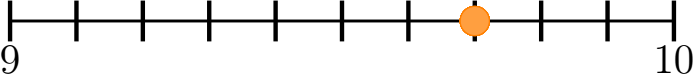
\includegraphics[width=180px]{../images/recta_num_9.7.png}   \hfill \fillin[\fbox{9.7 }][0in] \\
				\part 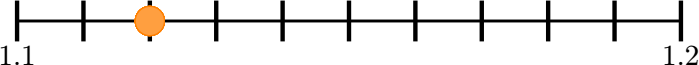
\includegraphics[width=180px]{../images/recta_num_1.12.png}  \hfill \fillin[\fbox{1.12}][0in] \\
				\part 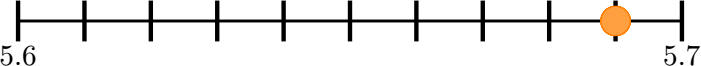
\includegraphics[width=180px]{../images/recta_num_5.69.png}  \hfill \fillin[\fbox{5.69}][0in] \\
				\part 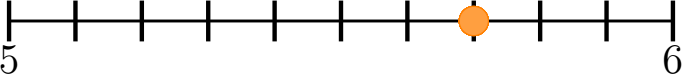
\includegraphics[width=180px]{../images/recta_num_5.7.png}   \hfill \fillin[\fbox{5.7 }][0in] \\
				\part 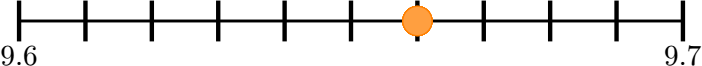
\includegraphics[width=180px]{../images/recta_num_9.66.png}  \hfill \fillin[\fbox{9.66}][0in] \\
				\part 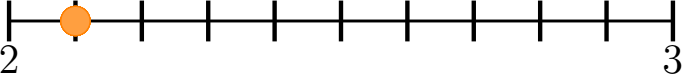
\includegraphics[width=180px]{../images/recta_num_2.1.png}   \hfill \fillin[\fbox{2.1 }][0in] \\
			\end{parts}
		\end{multicols}
	}

	% \subsection*{\ifprintanswers{Porcentaje como decimales             }

	\questionboxed[2]{Escribe los siguientes porcentajes como números decimales:

		\begin{multicols}{4}
			\begin{parts}
				\part $14\%=$ \fillin[\fbox{0.14}][0cm] \\
				\part $73\%=$ \fillin[\fbox{0.73}][0cm] \\
				\part $15\%=$ \fillin[\fbox{0.15}][0cm] \\
				\part $85\%=$ \fillin[\fbox{0.85}][0cm] \\
				\part $91\%=$ \fillin[\fbox{0.91}][0cm] \\
				\part $19\%=$ \fillin[\fbox{0.19}][0cm] \\
				\part $ 9\%=$ \fillin[\fbox{0.09}][0cm] \\
				\part $42\%=$ \fillin[\fbox{0.42}][0cm] \\
				\part $25\%=$ \fillin[\fbox{0.25}][0cm] \\
				\part $ 3\%=$ \fillin[\fbox{0.03}][0cm] \\
				\part $ 8\%=$ \fillin[\fbox{0.08}][0cm] \\
				\part $ 2\%=$ \fillin[\fbox{0.02}][0cm] \\
			\end{parts}
		\end{multicols}
	}

	% \subsection*{\ifprintanswers{Porcentaje de números                 }

	\questionboxed[2]{Calcula los porentajes de los siguientes números:

		\begin{multicols}{2}
			\begin{parts}
				\part ¿Cuál es el 80\% de 660?   \hfill \fillin[\fbox{528}][0cm]
				\part ¿Cuál es el 20\% de 50?    \hfill \fillin[\fbox{10}][0cm]
				\part ¿Cuál es el 50\% de 862?   \hfill \fillin[\fbox{431}][0cm]
				\part ¿Cuál es el 30\% de 300?   \hfill \fillin[\fbox{90}][0cm]
				\part ¿Cuál es el 20\% de 415?   \hfill \fillin[\fbox{83}][0cm]
				\part ¿Cuál es el 12\% de 338?   \hfill \fillin[\fbox{40.56}][0cm]
				\part ¿Cuál es el 15\% de 711?   \hfill \fillin[\fbox{106.65}][0cm]
				\part ¿Cuál es el 80\% de 1260?  \hfill \fillin[\fbox{1008}][0cm]
			\end{parts}
		\end{multicols}
	}

	% \subsection*{\ifprintanswers{Conversión de decimales a fracciones  }

	\questionboxed[2]{Convierte los siguientes números decimales a una fracción simplificada a su mínima expresión:

		\begin{multicols}{4}
			\begin{parts}
				\part $0.248=$ \fillin[\fbox{$\dfrac{31}{125}$}][0cm]
				\part $0.46=$  \fillin[\fbox{$\dfrac{23}{50}$}][0cm]
				\part $0.24=$  \fillin[\fbox{$\dfrac{6}{25}$}][0cm]
				\part $0.9=$   \fillin[\fbox{$\dfrac{9}{10}$}][0cm]
				\part $0.115=$ \fillin[\fbox{$\dfrac{23}{200}$}][0cm]
				\part $0.66=$  \fillin[\fbox{$\dfrac{33}{50}$}][0cm]
				\part $0.56=$  \fillin[\fbox{$\dfrac{14}{25}$}][0cm]
				\part $0.58=$  \fillin[\fbox{$\dfrac{29}{50}$}][0cm]
			\end{parts}
		\end{multicols}
	}

	% \subsection*{\ifprintanswers{Conversión de fracciones a decimales  }  

	\questionboxed[2]{Convierte las siguientes fracciones a decimal:

		\begin{multicols}{5}
			\begin{parts}
				\part $\dfrac{2}{9} =$   \fillin[\fbox{$0.\overline{2}$}][0cm]\\
				\part $\dfrac{1}{4} =$   \fillin[\fbox{$0.25$}][0cm]\\
				\part $\dfrac{2}{3} =$   \fillin[\fbox{$0.\overline{6}$}][0cm]\\
				\part $\dfrac{7}{8} =$   \fillin[\fbox{$0.875$}][0cm]\\
				\part $\dfrac{1}{9} =$   \fillin[\fbox{$0.\overline{1}$}][0cm]\\
				\part $\dfrac{6}{8} =$   \fillin[\fbox{$0.75$}][0cm]\\
				\part $\dfrac{7}{20}=$   \fillin[\fbox{$0.35$}][0cm]\\
				\part $\dfrac{5}{8} =$   \fillin[\fbox{$0.625$}][0cm]\\
				\part $\dfrac{2}{10}=$   \fillin[\fbox{$0.2$}][0cm]\\
				\part $\dfrac{5}{6} =$   \fillin[\fbox{$0.8\overline{3}$}][0cm]\\
			\end{parts}
		\end{multicols}
	}


	\addcontentsline{toc}{subsection}{Introducción a las fracciones}
	\subsection*{Introducción a las fracciones}

	% \subsection*{\ifprintanswers{Clasificación de fracciones           }
	\questionboxed[2]{Clasifica las siguientes fracciones en propias, impropias o mixtas:

		\begin{multicols}{4}
			\begin{parts}
				\part $\dfrac{5}{6}$   \fillin[Propia][1in]     \\[0.5em]
				\part $5\dfrac{5}{11}$ \fillin[Mixta][1in]      \\[0.5em]
				\part $\dfrac{13}{12}$   \fillin[Impropia][1in] \\[0.5em]
				\part $1\dfrac{2}{15}$  \fillin[Mixta][1in]     \\[0.5em]
				\part $\dfrac{42}{43}$   \fillin[Propia][1in]   \\[0.5em]
				\part $\dfrac{16}{9}$   \fillin[Impropia][1in]  \\[0.5em]
				\part $\dfrac{7}{3}$   \fillin[Impropia][1in]   \\[0.5em]
				\part $3\dfrac{2}{9}$  \fillin[Mixta][1in]      \\[0.5em]
				\part $\dfrac{3}{2}$   \fillin[Impropia][1in]   \\[0.5em]
				\part $1\dfrac{2}{3}$  \fillin[Mixta][1in]      \\[0.5em]
				\part $\dfrac{7}{8}$   \fillin[Propia][1in]     \\[0.5em]
				\part $\dfrac{6}{5}$   \fillin[Impropia][1in]   \\[0.5em]
			\end{parts}
		\end{multicols}
	}

	% \subsection*{\ifprintanswers{Nombre de fracciones                       }\else{}\fi}

	\questionboxed[2]{Escribe la fracción que corresponda en cada inciso:

		\begin{parts}
			\part ¿Cómo se escribe numéricamente la fracción \textbf{siete catorceavos}?    \fillin[$\dfrac{7}{14}$][0in]
			\part ¿Cómo se escribe numéricamente la fracción \textbf{ocho onceavos}?   \fillin[$\dfrac{8}{11}$][0in]
			\part ¿Cómo se escribe numéricamente la fracción \textbf{doce séptimos}?    \fillin[$\dfrac{12}{7}$][0in]
			\part ¿Cómo se escribe numéricamente la fracción \textbf{nueve treceavos}?     \fillin[$\dfrac{9}{13}$][0in]
		\end{parts}
	}

	% \subsection*{\ifprintanswers{Representación de fracciones}\else{}\fi}
	\questionboxed[2]{Escribe sobre la línea la fracción que representa cada imagen:

		\begin{multicols}{4}
			\begin{parts}
				\part 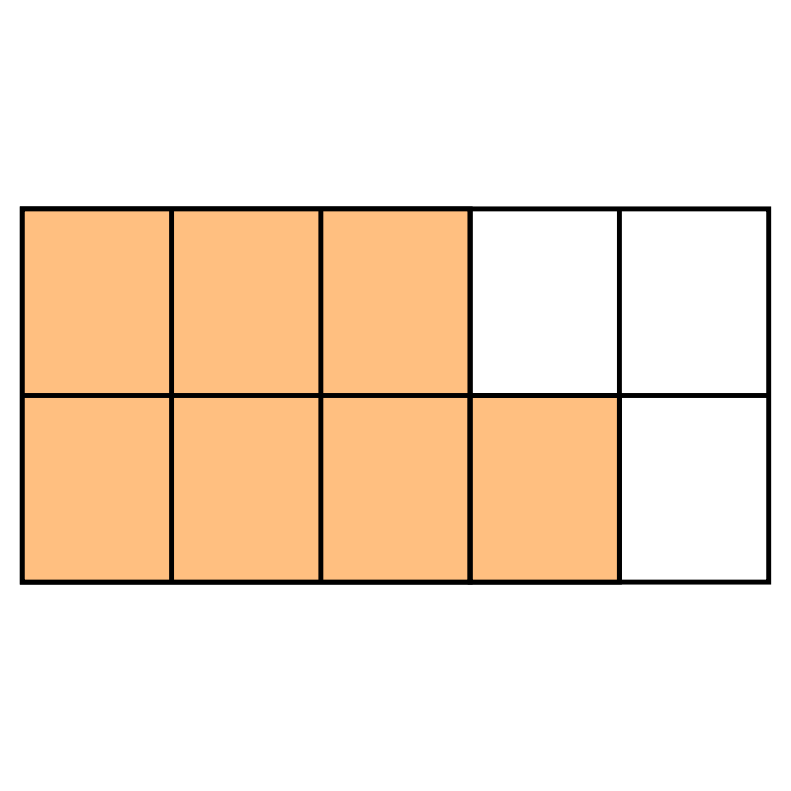
\includegraphics[width=50px]{../images/imagen_frac_5prim_7|10.png} \fillin[\fbox{$\dfrac{7}{10}$}][0in] \\[-0.5em]
				\part 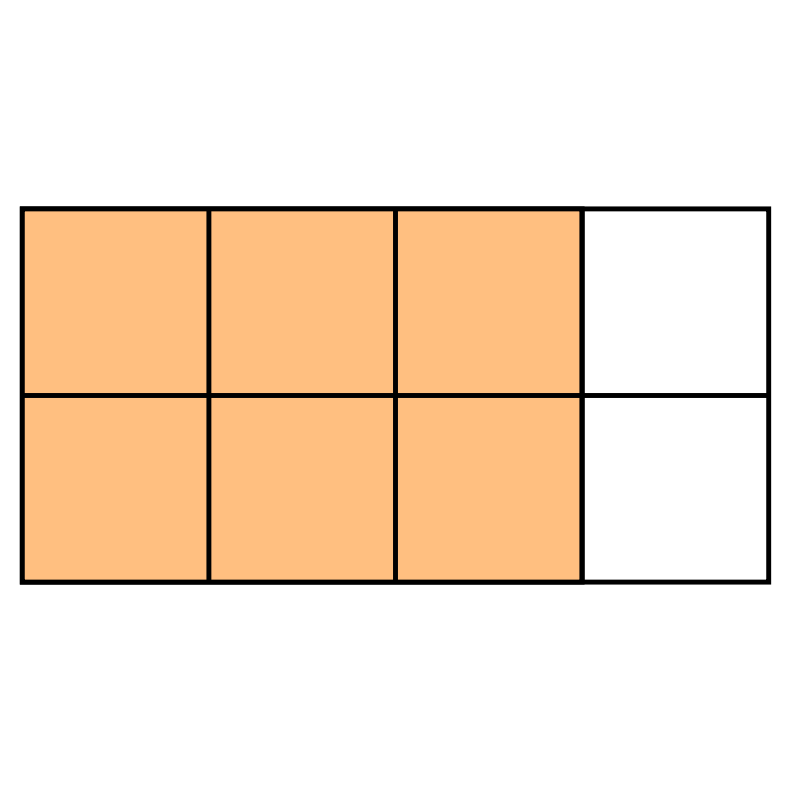
\includegraphics[width=50px]{../images/imagen_frac_5prim_6|8.png} \fillin[\fbox{$\dfrac{6}{8}$}][0in] \\[-0.5em]
				\part 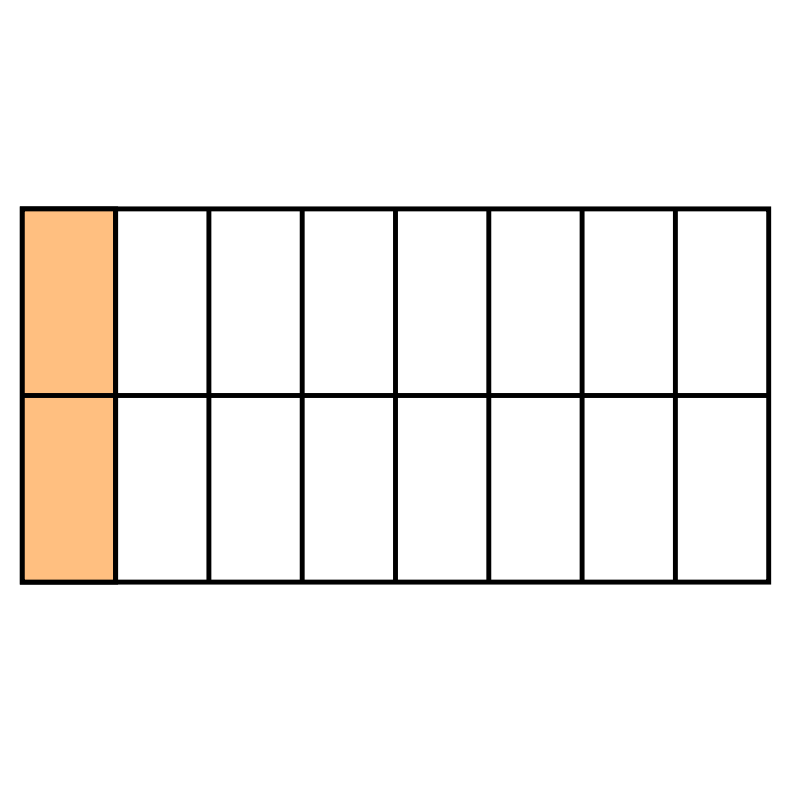
\includegraphics[width=50px]{../images/imagen_frac_5prim_2|16.png} \fillin[\fbox{$\dfrac{2}{16}$}][0in] \\[-0.5em]
				\part 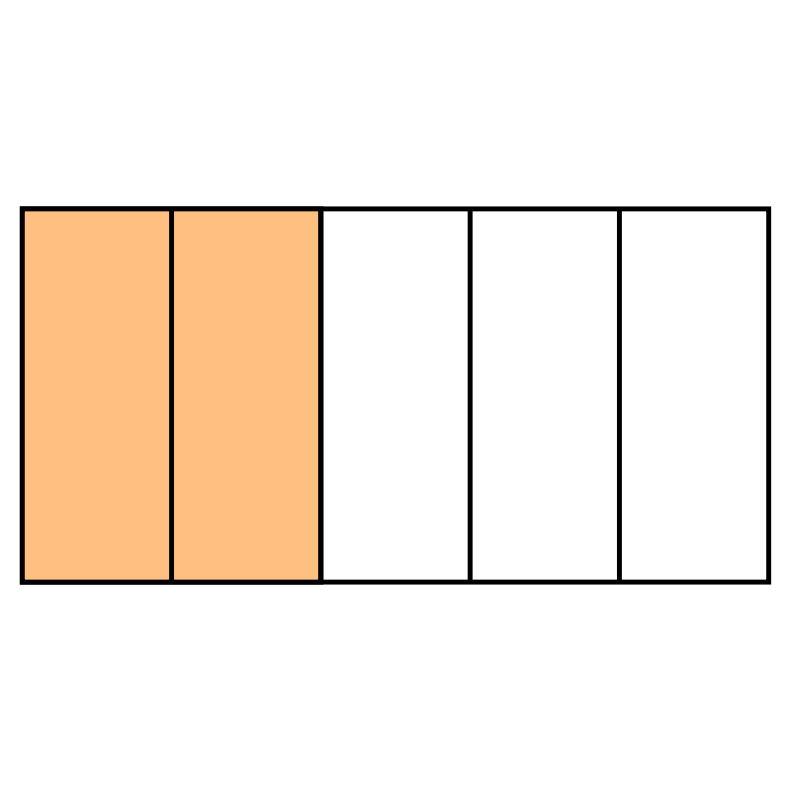
\includegraphics[width=50px]{../images/imagen_frac_5prim_2|5.png} \fillin[\fbox{$\dfrac{2}{5}$}][0in] \\[-0.5em]
				\part 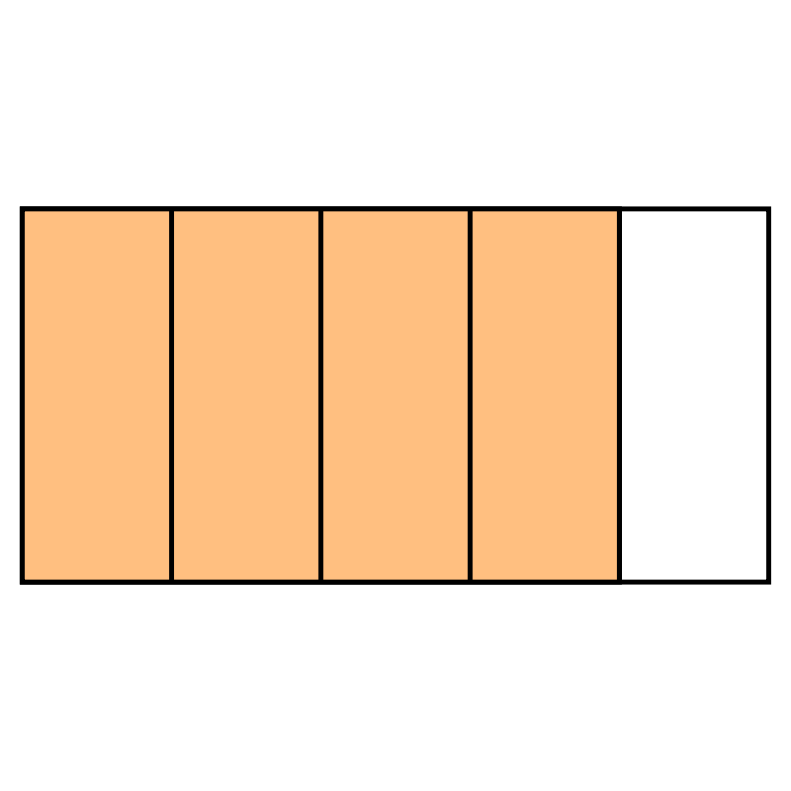
\includegraphics[width=50px]{../images/imagen_frac_5prim_4|5.png} \fillin[\fbox{$\dfrac{4}{5}$}][0in] \\[-0.5em]
				\part 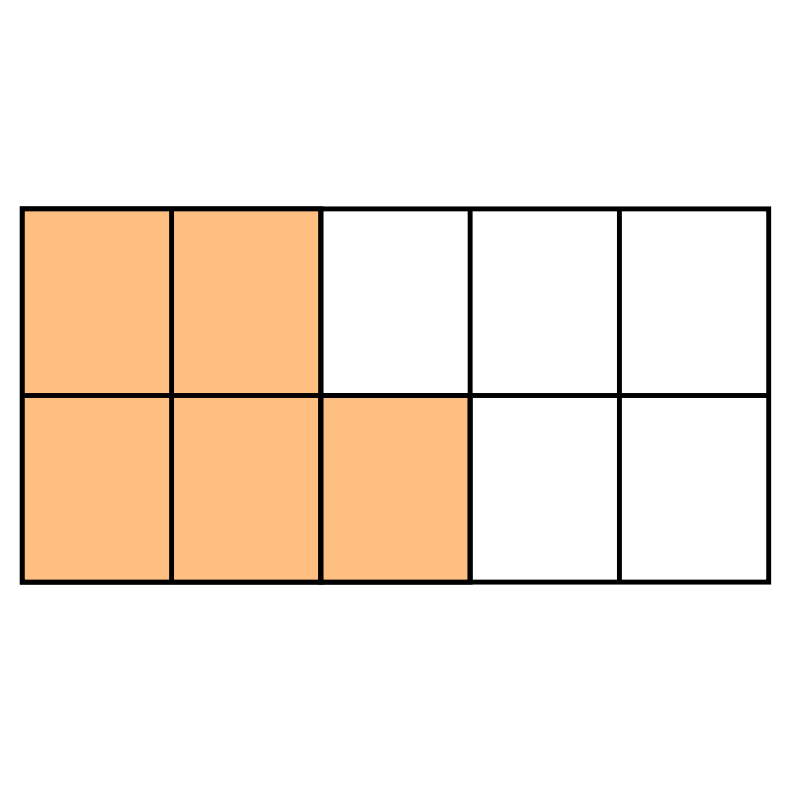
\includegraphics[width=50px]{../images/imagen_frac_5prim_5|10.png} \fillin[\fbox{$\dfrac{5}{10}$}][0in] \\[-0.5em]
				\part 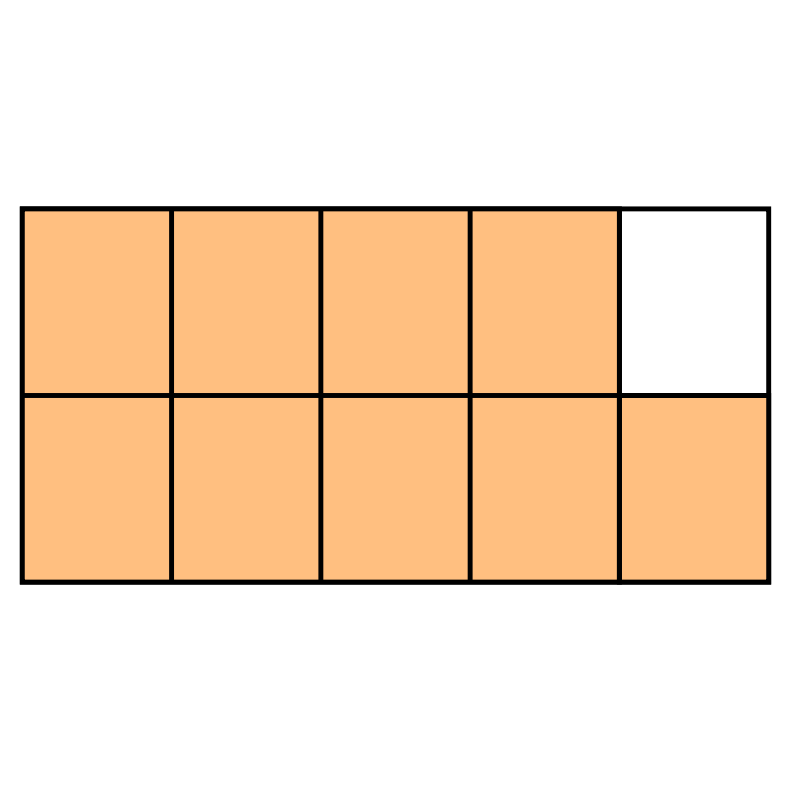
\includegraphics[width=50px]{../images/imagen_frac_5prim_9|10.png} \fillin[\fbox{$\dfrac{9}{10}$}][0in] \\[-0.5em]
				\part 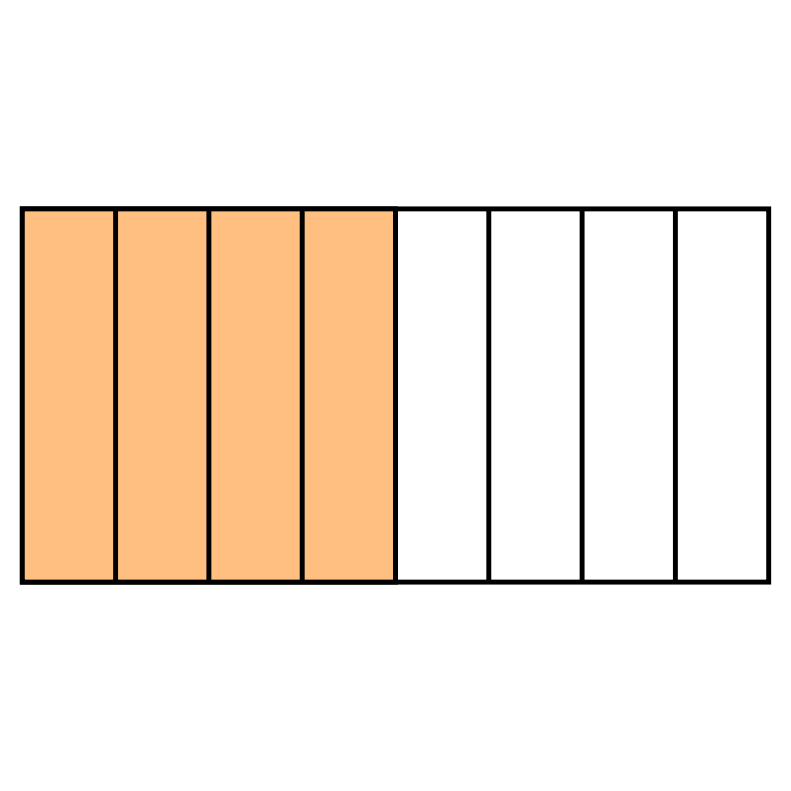
\includegraphics[width=50px]{../images/imagen_frac_5prim_4|8.png} \fillin[\fbox{$\dfrac{4}{8}$}][0in] \\[-0.5em]
				\part 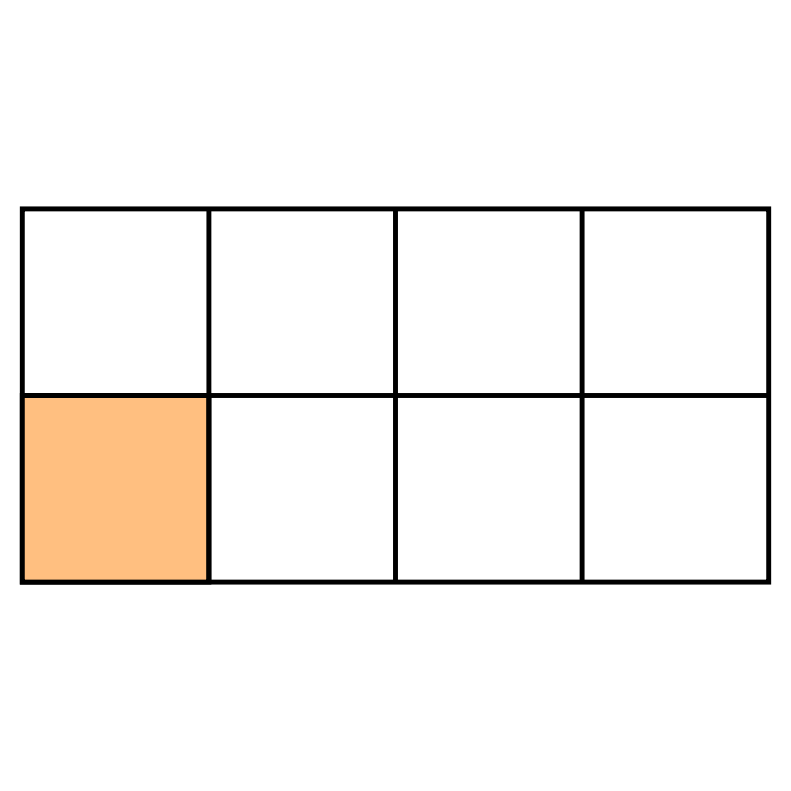
\includegraphics[width=50px]{../images/imagen_frac_5prim_1|8.png} \fillin[\fbox{$\dfrac{1}{8}$}][0in] \\[-0.5em]
				\part 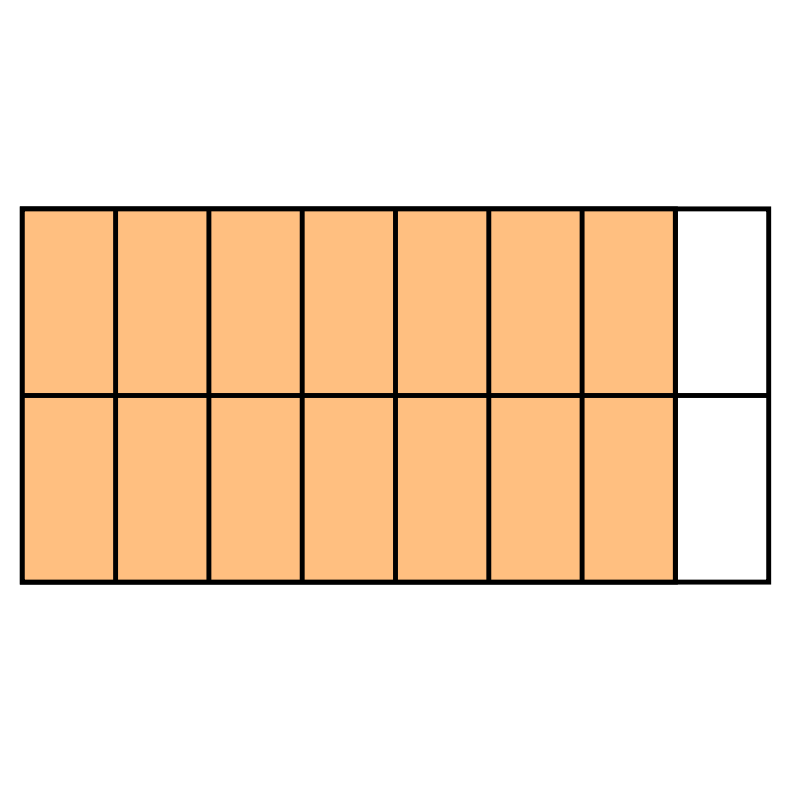
\includegraphics[width=50px]{../images/imagen_frac_5prim_14|16.png} \fillin[\fbox{$\dfrac{14}{16}$}][0in] \\[-0.5em]
				\part 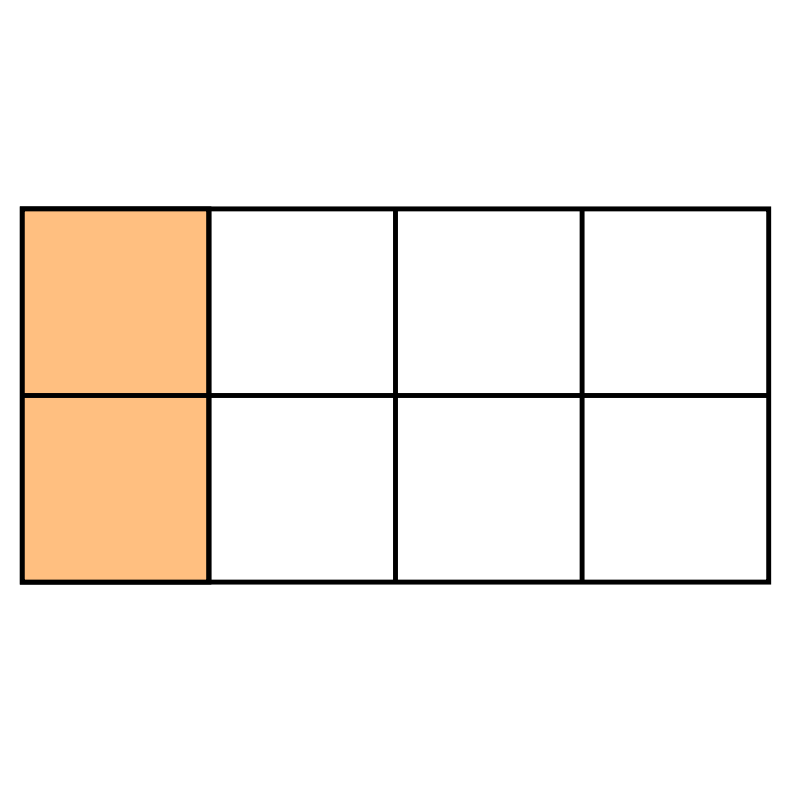
\includegraphics[width=50px]{../images/imagen_frac_5prim_2|8.png} \fillin[\fbox{$\dfrac{2}{8}$}][0in] \\[-0.5em]
				\part 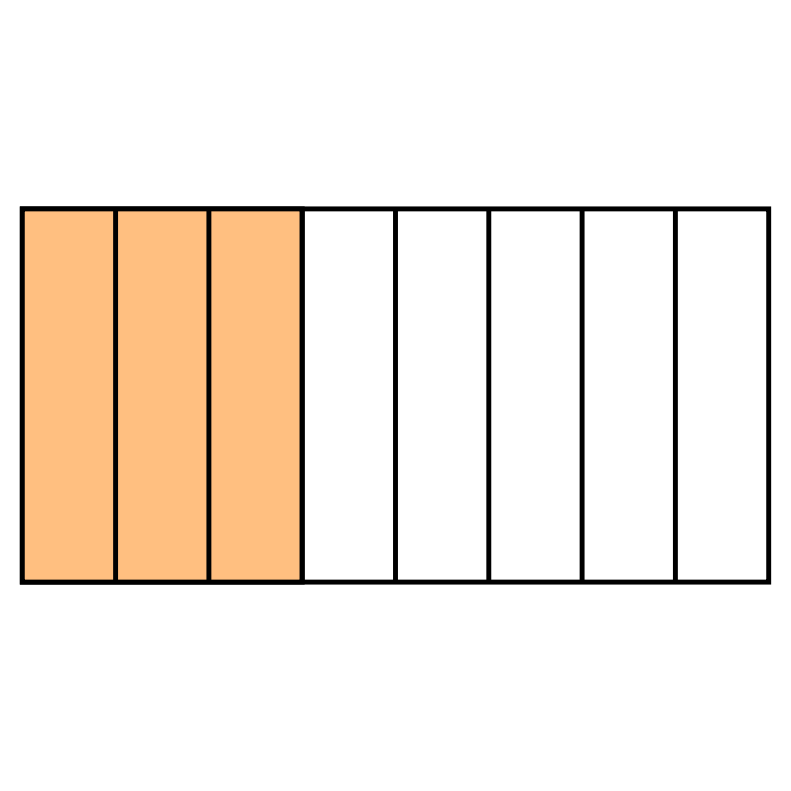
\includegraphics[width=50px]{../images/imagen_frac_5prim_3|8.png} \fillin[\fbox{$\dfrac{3}{8}$}][0in] \\[-0.5em]
				\part 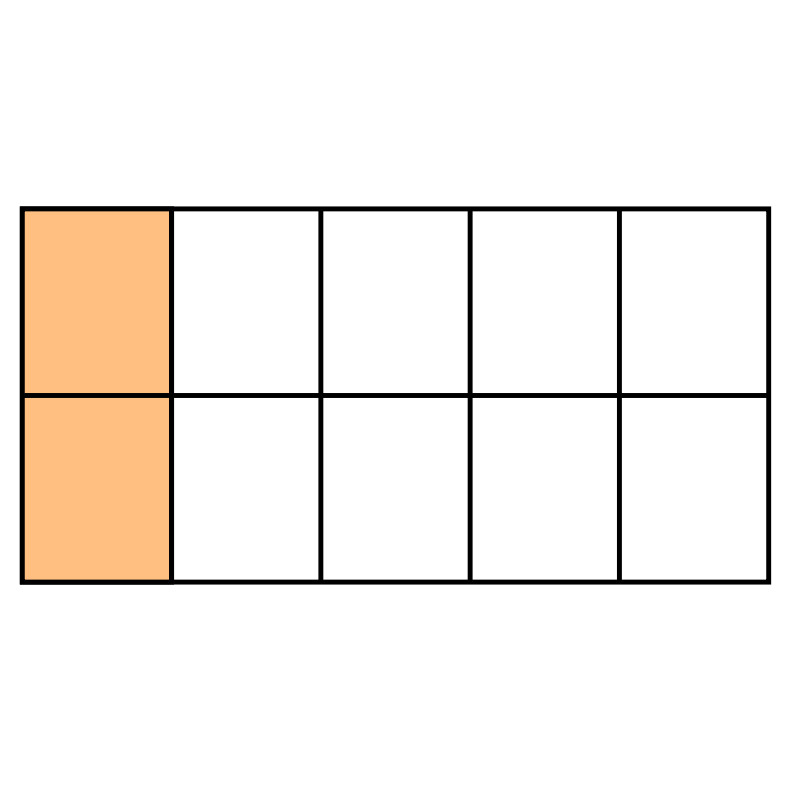
\includegraphics[width=50px]{../images/imagen_frac_5prim_2|10.png} \fillin[\fbox{$\dfrac{2}{10}$}][0in] \\[-0.5em]
				\part 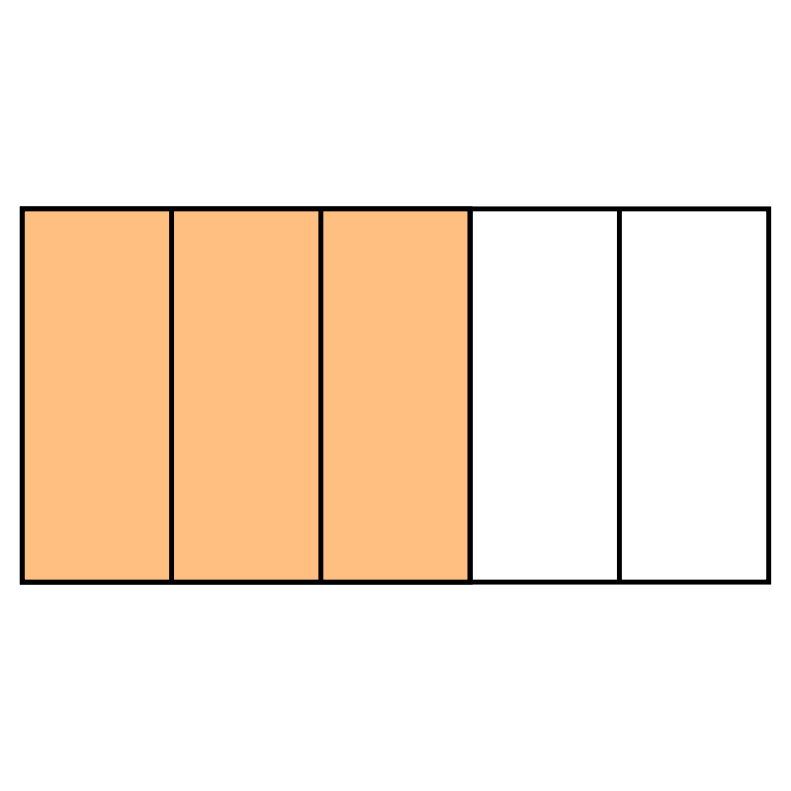
\includegraphics[width=50px]{../images/imagen_frac_5prim_3|5.png} \fillin[\fbox{$\dfrac{3}{5}$}][0in] \\[-0.5em]
				\part 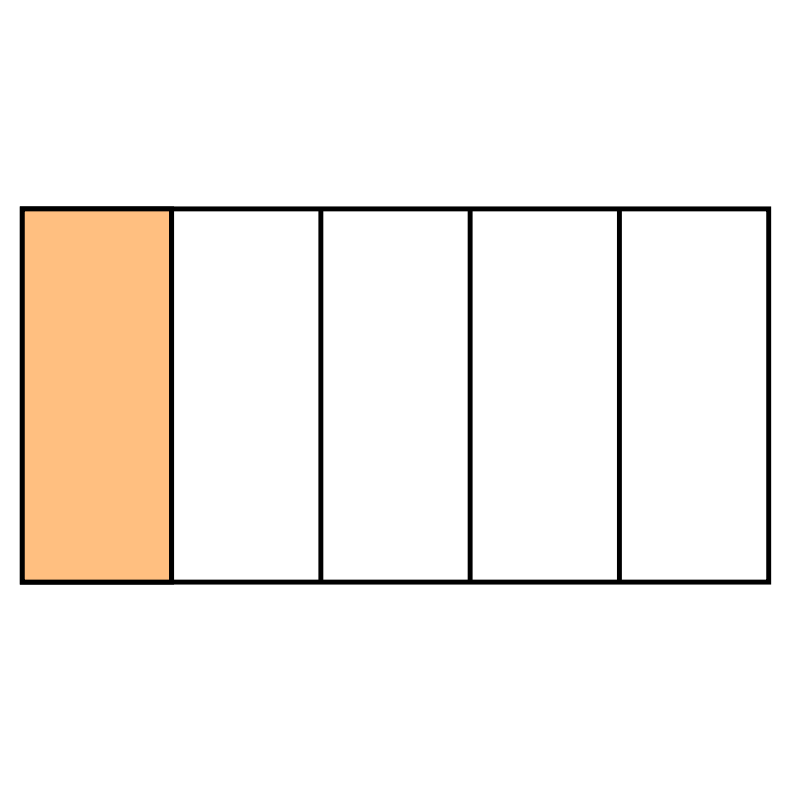
\includegraphics[width=50px]{../images/imagen_frac_5prim_1|5.png} \fillin[\fbox{$\dfrac{1}{5}$}][0in] \\[-0.5em]
				\part 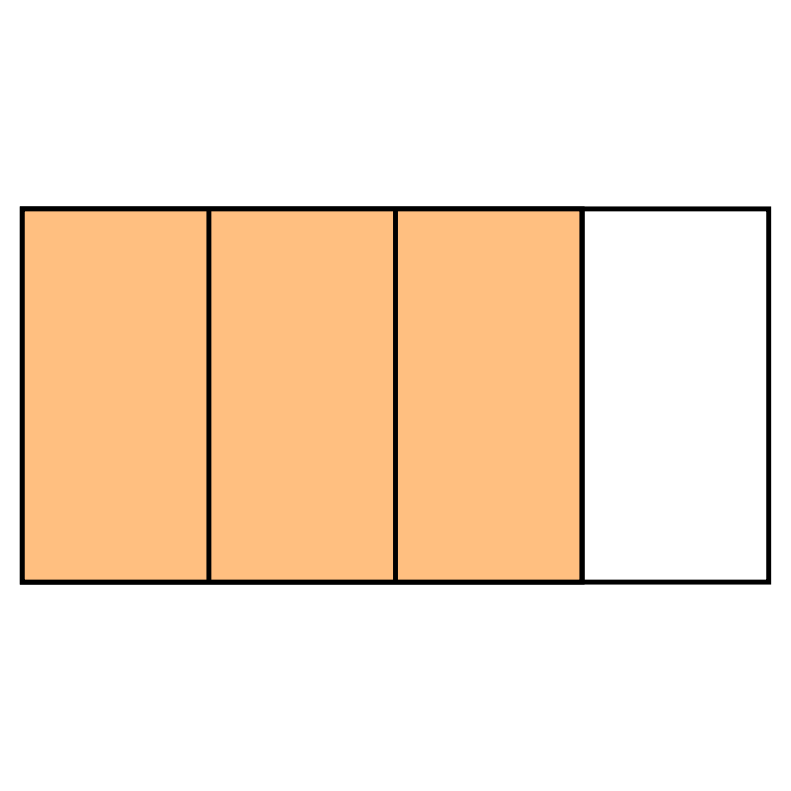
\includegraphics[width=50px]{../images/imagen_frac_5prim_3|4.png} \fillin[\fbox{$\dfrac{3}{4}$}][0in] \\[-0.5em]


			\end{parts}
		\end{multicols}
	}


	% \subsection*{\ifprintanswers{Fracciones en la recta numérica}
	% \subsection*{\ifprintanswers{Decimales en la recta númerica        }
	\questionboxed[2]{Escribe la fracción que representa el punto en la recta numérica de cada imagen:

		\begin{multicols}{2}
			\begin{parts}
				\part 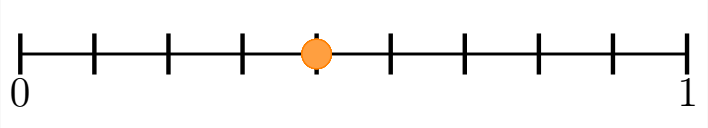
\includegraphics[width=180px]{../images/recta_num_frac4|9.png}   \hfill \fillin[\fbox{$\dfrac{ 4}{9 }$}][0in] \\
				\part 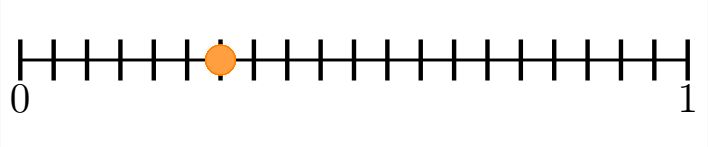
\includegraphics[width=180px]{../images/recta_num_frac6|20.png}  \hfill \fillin[\fbox{$\dfrac{ 6}{20}$}][0in] \\
				\part 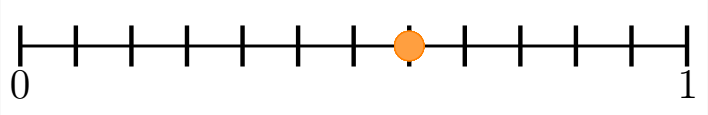
\includegraphics[width=180px]{../images/recta_num_frac7|12.png}  \hfill \fillin[\fbox{$\dfrac{ 7}{12}$}][0in] \\
				\part 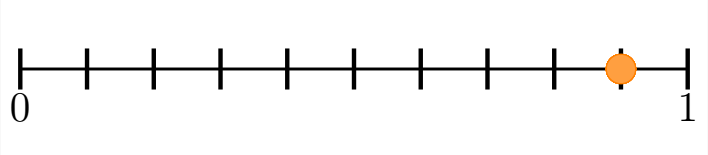
\includegraphics[width=180px]{../images/recta_num_frac9|10.png}  \hfill \fillin[\fbox{$\dfrac{ 9}{10}$}][0in] \\
				\part 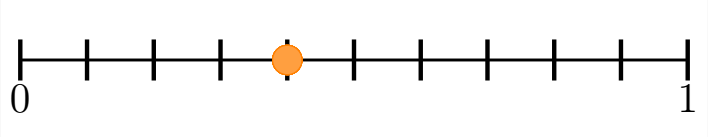
\includegraphics[width=180px]{../images/recta_num_frac4|10.png}  \hfill \fillin[\fbox{$\dfrac{ 4}{10}$}][0in] \\
				\part 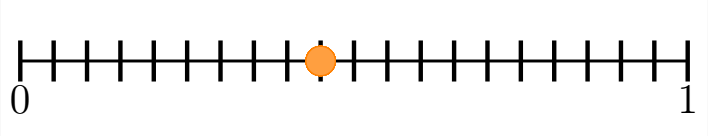
\includegraphics[width=180px]{../images/recta_num_frac9|20.png}  \hfill \fillin[\fbox{$\dfrac{ 9}{20}$}][0in] \\
				\part 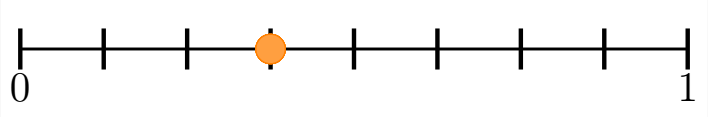
\includegraphics[width=180px]{../images/recta_num_frac3|8.png}   \hfill \fillin[\fbox{$\dfrac{ 3}{8 }$}][0in] \\
				\part 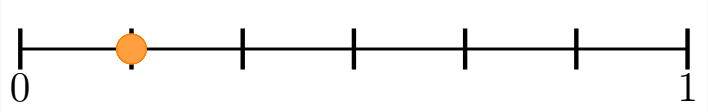
\includegraphics[width=180px]{../images/recta_num_frac1|6.png}   \hfill \fillin[\fbox{$\dfrac{ 1}{6 }$}][0in] \\
				\part 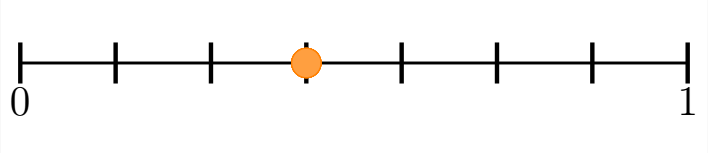
\includegraphics[width=180px]{../images/recta_num_frac3|7.png}   \hfill \fillin[\fbox{$\dfrac{ 3}{7 }$}][0in] \\
				\part 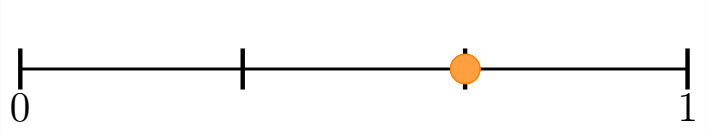
\includegraphics[width=180px]{../images/recta_num_frac2|3.png}   \hfill \fillin[\fbox{$\dfrac{ 2}{3 }$}][0in] \\
			\end{parts}
		\end{multicols}
	}



	% \subsection*{\ifprintanswers{Conversión de fracciones}
	\questionboxed[2]{Convierte la siguientes fracciones mixtas a impropias y viseversa:

		\begin{multicols}{3}
			\begin{parts}
				\part $4\dfrac{2}{3}= $  \fillin[$\dfrac{14}{3}$][0in]\\[0.5em]
				\part $\dfrac{13}{3}= $  \fillin[$4\dfrac{1}{3}$][0in]\\[0.5em]
				\part $2\dfrac{3}{10}= $ \fillin[$\dfrac{23}{10}$][0in]\\[0.5em]
				\part $\dfrac{43}{10}= $ \fillin[$4\dfrac{3}{10}$][0in]\\[0.5em]
				\part $5\dfrac{1}{5}= $  \fillin[$\dfrac{26}{5}$][0in]\\[0.5em]
				\part $\dfrac{51}{5}= $  \fillin[$10\dfrac{1}{5}$][0in]\\[0.5em]
			\end{parts}
		\end{multicols}
	}



	\addcontentsline{toc}{subsection}{Suma y resta de fracciones}
	\subsection*{Suma y resta de fracciones}
	% \subsection*{\ifprintanswers{Simplificación de fracciones          }
	\questionboxed[2]{Simplifica a su mínima expresión las siguientes fracciones usando el máximo común divisor:

		\begin{multicols}{5}
			\begin{parts}
				\part $\dfrac{12}{48}= $  \fillin[$\dfrac{1}{4}$][0in]\\[0.5em]
				\part $\dfrac{6}{24}= $  \fillin[$\dfrac{1}{4}$][0in]\\[0.5em]
				\part $\dfrac{16}{36}= $  \fillin[$\dfrac{4}{9}$][0in]\\[0.5em]
				\part $\dfrac{4}{40}= $  \fillin[$\dfrac{1}{10}$][0in]\\[0.5em]
				\part $\dfrac{4}{20}= $  \fillin[$\dfrac{1}{5}$][0in]\\[0.5em]
				\part $\dfrac{2}{30}= $  \fillin[$\dfrac{1}{15}$][0in]\\[0.5em]
				\part $\dfrac{6}{36}= $  \fillin[$\dfrac{1}{6}$][0in]\\[0.5em]
				\part $\dfrac{5}{25}= $  \fillin[$\dfrac{1}{5}$][0in]\\[0.5em]
				\part $\dfrac{6}{30}= $  \fillin[$\dfrac{1}{5}$][0in]\\[0.5em]
				\part $\dfrac{2}{12}= $  \fillin[$\dfrac{1}{6}$][0in]\\[0.5em]
				\part $\dfrac{4}{16}= $  \fillin[$\dfrac{1}{4}$][0in]\\[0.5em]
				\part $\dfrac{15}{20}= $  \fillin[$\dfrac{3}{4}$][0in]\\[0.5em]
				\part $\dfrac{5}{50}= $  \fillin[$\dfrac{1}{10}$][0in]\\[0.5em]
				\part $\dfrac{6}{10}= $  \fillin[$\dfrac{3}{5}$][0in]\\[0.5em]
				\part $\dfrac{3}{18}= $  \fillin[$\dfrac{1}{6}$][0in]\\[0.5em]
			\end{parts}
		\end{multicols}
	}


	% \subsection*{\ifprintanswers{Suma y resta con denominadores iguales}
	% \subsection*{\ifprintanswers{Suma con denominadores diferentes     }
	% \subsection*{\ifprintanswers{Resta con denominadores diferentes    }
	% \subsection*{\ifprintanswers{Sumas y restas con fracciones mixtas  }

	\questionboxed[4]{Realiza las siguientes operaciones de suma y resta de fracciones:

		\begin{multicols}{3}
			\begin{parts}
				\part $\dfrac{3}{5}+\dfrac{4}{5}=$ \fillin[$\dfrac{7}{5} = 1\dfrac{2}{5}$][0in] \\[1em]
				\part $\dfrac{3}{10}+\dfrac{4}{5}=$ \fillin[$\dfrac{11}{10} = 1\dfrac{1}{10}$][0in] \\[1em]
				\part $\dfrac{9}{10}+\dfrac{2}{3}=$ \fillin[$1\dfrac{17}{30}$][0in] \\[1em]
				\part $\dfrac{13}{6}-\dfrac{5}{6}=$ \fillin[$\dfrac{8}{6}=\dfrac{4}{3}$][0in] \\[1em]
				\part $1\dfrac{1}{2}+1\dfrac{2}{3}=$ \fillin[$3\dfrac{1}{6}$][0in] \\[1em]
				\part $\dfrac{3}{4}-\dfrac{2}{5}=$ \fillin[$\dfrac{7}{20}$][0in] \\[1em]
				\part $\dfrac{5}{6}+\dfrac{1}{12}=$ \fillin[$\dfrac{11}{12}$][0in] \\[1em]
				\part $\dfrac{12}{7}-\dfrac{5}{7}=$ \fillin[$\dfrac{7}{7}=1$][0in] \\[1em]
				\part $\dfrac{2}{3}-\dfrac{2}{5}=$ \fillin[$\dfrac{4}{15}$][0in] \\[1em]
				\part $2\dfrac{1}{2}-1\dfrac{1}{3}=$ \fillin[$1\dfrac{1}{6}$][0in] \\[1em]
				\part $\dfrac{1}{3}-\dfrac{1}{4}=$ \fillin[$\dfrac{1}{12}$][0in] \\[1em]
				\part $1\dfrac{1}{8}+1\dfrac{7}{8}=$ \fillin[$2\dfrac{8}{8} = 3$][0in] \\[1em]
				\part $\dfrac{3}{8}+\dfrac{7}{10}=$ \fillin[$\dfrac{43}{40} = 1\dfrac{3}{40}$][0in] \\[1em]
				\part $\dfrac{3}{4}-\dfrac{1}{8}=$ \fillin[$\dfrac{5}{8}$][0in] \\[1em]
				\part $3\dfrac{3}{4}-2\dfrac{2}{3}=$ \fillin[$1\dfrac{1}{12}$][0in] \\[1em]
			\end{parts}
		\end{multicols}
	}


	\addcontentsline{toc}{subsection}{Multiplicación y división de fracciones}
	\subsection*{Multiplicación y división de fracciones}
	% \subsection*{\ifprintanswers{Multiplicación de fracciones          }
	% \subsection*{\ifprintanswers{División de fracciones                }
	% \subsection*{\ifprintanswers{Multiplicación y división con enteros }
	% \subsection*{\ifprintanswers{Multiplicación con fracciones mixtas  }
	% \subsection*{\ifprintanswers{División con fracciones mixtas        }

	\questionboxed[5]{Realiza las siguientes operaciones de multiplicación y división de fracciones (Expresa tu resultadocomo una \textbf{fracción simplificada}):

		\begin{multicols}{4}
			\begin{parts}
				\part $\dfrac{7}{9}\times\dfrac{12}{17}=$ \fillin[$\dfrac{28}{51}$][0in]   \\[1em]
				\part $\dfrac{2}{7}\divisionsymbol\dfrac{2}{5}=$ \fillin[$\dfrac{5}{7}$][0in]   \\[1em]
				\part $3\times\dfrac{5}{4}=$ \fillin[$\dfrac{15}{4}$][0in]   \\[1em]
				\part $1\dfrac{1}{4}\times 4\dfrac{5}{8}=$ \fillin[$\dfrac{185}{32}$][0in]   \\[1em]
				\part $\dfrac{5}{6}\times\dfrac{4}{5}=$ \fillin[$\dfrac{2}{3}$][0in]   \\[1em]
				\part $\dfrac{4}{7}\divisionsymbol\dfrac{5}{6}=$ \fillin[$\dfrac{24}{35}$][0in]   \\[1em]
				\part $\dfrac{7}{6}\times 6=$ \fillin[$\dfrac{21}{2}$][0in]   \\[1em]
				\part $3\dfrac{1}{3}\times 2\dfrac{2}{5}=$ \fillin[$8$][0in]   \\[1em]
				\part $\dfrac{3}{7}\times\dfrac{5}{6}=$ \fillin[$\dfrac{5}{14}$][0in]   \\[1em]
				\part $\dfrac{7}{8}\divisionsymbol\dfrac{5}{4}=$ \fillin[$\dfrac{7}{10}$][0in]   \\[1em]
				\part $\dfrac{2}{5}\divisionsymbol 5=$ \fillin[$\dfrac{2}{25}$][0in]   \\[1em]
				\part $6\dfrac{1}{2}\divisionsymbol 1\dfrac{5}{7}=$ \fillin[$\dfrac{91}{24}$][0in]   \\[1em]
				\part $\dfrac{5}{8}\times\dfrac{4}{5}=$ \fillin[$\dfrac{1}{2}$][0in]   \\[1em]
				\part $\dfrac{6}{7}\divisionsymbol\dfrac{1}{3}=$ \fillin[$\dfrac{18}{7}$][0in]   \\[1em]
				\part $4\divisionsymbol\dfrac{3}{5}=$ \fillin[$\dfrac{20}{3}$][0in]   \\[1em]
				\part $2\dfrac{2}{3}\divisionsymbol 1\dfrac{3}{4}=$ \fillin[$\dfrac{32}{21}$][0in]   \\[1em]
			\end{parts}
		\end{multicols}
	}


	\addcontentsline{toc}{subsection}{MCD y MCM}
	\subsection*{MCD y MCM}


	% \subsection*{\ifprintanswers{Fracciones equivalentes               }

	\questionboxed[2]{Indica si las siguientes fracciones son equivalentes o no:

		\begin{multicols}{2}
			\begin{parts}

				\part $\dfrac{1}{2}=\dfrac{4}{6}$\qquad
				\begin{oneparcheckboxes}
					\choice Sí
					\CorrectChoice No
				\end{oneparcheckboxes}

				\part $\dfrac{4}{5}=\dfrac{8}{10}$\qquad
				\begin{oneparcheckboxes}
					\CorrectChoice Sí
					\choice No
				\end{oneparcheckboxes}

				\part $\dfrac{1}{8}=\dfrac{4}{16}$\qquad
				\begin{oneparcheckboxes}
					\choice Sí
					\CorrectChoice No
				\end{oneparcheckboxes}

				\part $\dfrac{1}{5}=\dfrac{5}{10}$\qquad
				\begin{oneparcheckboxes}
					\choice Sí
					\CorrectChoice No
				\end{oneparcheckboxes}

				\part $\dfrac{1}{10}=\dfrac{3}{30}$\qquad
				\begin{oneparcheckboxes}
					\CorrectChoice Sí
					\choice No
				\end{oneparcheckboxes}

				\part $\dfrac{1}{4}=\dfrac{2}{4}$\qquad
				\begin{oneparcheckboxes}
					\choice Sí
					\CorrectChoice No
				\end{oneparcheckboxes}

				\part $\dfrac{1}{5}=\dfrac{10}{25}$\qquad
				\begin{oneparcheckboxes}
					\choice Sí
					\CorrectChoice No
				\end{oneparcheckboxes}

				\part $\dfrac{3}{2}=\dfrac{12}{8}$\qquad
				\begin{oneparcheckboxes}
					\CorrectChoice Sí
					\choice No
				\end{oneparcheckboxes}

				\part $\dfrac{3}{6}=\dfrac{1}{3}$\qquad
				\begin{oneparcheckboxes}
					\choice Sí
					\CorrectChoice No
				\end{oneparcheckboxes}

				\part $\dfrac{18}{12}=\dfrac{9}{4}$\qquad
				\begin{oneparcheckboxes}
					\choice Sí
					\CorrectChoice No
				\end{oneparcheckboxes}
			\end{parts}
		\end{multicols}
	}

	% \subsection*{\ifprintanswers{Factores primos                       }

	\questionboxed[2]{Descomponer en factores primos cada uno de los siguientes números:

		\begin{multicols}{3}
			\begin{parts}
				\part $81=$    \fillin[$3 \times 3 \times 3 \times 3$][3.8cm] \\
				\part $34=$    \fillin[$2 \times 17$][3.8cm] \\
				\part $8=$     \fillin[$2 \times 2 \times 2$][3.8cm] \\
				\part $243=$   \fillin[$3 \times 3 \times 3 \times 3 \times 3$][3.8cm] \\
				\part $33=$    \fillin[$3 \times 11$][3.8cm] \\
				\part $150=$   \fillin[$2 \times 3 \times 5 \times 5$][3.8cm] \\
				\part $144=$   \fillin[$2 \times 2 \times 2 \times 2 \times 3 \times 3$][3.8cm] \\
				\part $55=$    \fillin[$5 \times 11$][3.8cm] \\
				\part $125=$   \fillin[$5 \times 5 \times 5$][3.8cm] \\
			\end{parts}
		\end{multicols}
	}

	% \subsection*{\ifprintanswers{Mínimo común múltiplo                 }

	% \subsection*{\ifprintanswers{Máximo común divisor                  }
	\questionboxed[4]{Calcula lo que se te pide en cada inciso:

		% \begin{multicols}{2}
		\begin{parts}
			\part Encuentra el mínimo común múltiplo de 2 y 9.     	\hfill\fillin[El MCM de 2 y 9 es 18.][0in] \\[0.8em]
			\part Encuentra el máximo común divisor de 5 y 15.     	\hfill\fillin[El MCD de 5 y 15 es 5.][0in] \\[0.8em]
			\part Encuentra el máximo común divisor de 33 y 121.   	\hfill\fillin[El MCD de 33 y 121 es 11.][0in] \\[0.8em]
			\part Encuentra el máximo común divisor de 25 y 100.   	\hfill\fillin[El MCD de 25 y 100 es 25.][0in] \\[0.8em]
			\part Encuentra el máximo común divisor de 18 y 36.    	\hfill\fillin[El MCD de 18 y 36 es 18.][0in] \\[0.8em]
			\part Encuentra el mínimo común múltiplo de 4 y 9.     	\hfill\fillin[El MCM de 4 y 9 es 36.][0in] \\[0.8em]
			\part Encuentra el mínimo común múltiplo de 6 y 7.     	\hfill\fillin[El MCM de 6 y 7 es 42.][0in] \\[0.8em]
			\part Encuentra el mínimo común múltiplo de 2, 3 y 4.  	\hfill\fillin[El MCM de 2, 3 y 4 es 12.][0in] \\[0.8em]
			\part Encuentra el máximo común divisor de 2 y 14.     	\hfill\fillin[El MCD de 2 y 14 es 2.][0in] \\[0.8em]
			\part Encuentra el mínimo común múltiplo de 12, 15 y 18.\hfill\fillin[El MCM de 12, 15 y 18 es 180.][0in] \\[0.8em]
		\end{parts}
		% \end{multicols}
	}

	% \subsection*{\ifprintanswers{Simplificación de fracciones          }
\end{questions}
\end{document}